%%%%%%%%%%%%%%%%%%%%%%%%%%%%%%%%%%%%%%%%%%%%%%%%%%%%%%%%%
%                                                       %
%  	     PRESENTACIÓN 1-Introduccion a LaTeX	%
%                                                       %
%%%%%%%%%%%%%%%%%%%%%%%%%%%%%%%%%%%%%%%%%%%%%%%%%%%%%%%%


\documentclass[xcolor=dvipsnames]{beamer}    %Inicio de presentación

%
% Paquetes que pueden serte de utilidad (rec = recomendado, opc = opcional)
%
\usepackage{fancyhdr}          % (rec)  permite cambiar varios par�metros de las cabeceras y pi�s de p�gina
\usepackage{fancyvrb}		% (rec) permite cambiar parámetros del texto
% literal (entorno verbatim)
\usepackage{courier}           % (opc)  usa esta fuente por defecto
\usepackage[spanish]{babel}   % (rec)  da soporte para castellano a LaTeX
\usepackage[utf8]{inputenc}    % (rec) soporte para tildes
%\usepackage{setspace}          % (opc)  permite cambiar el espaciado entre l�neas
%\usepackage{longtable}         % (opc)  permite que las tablas ocupen varias p�ginas
%\usepackage{lscape}            % (opc)  permite el uso del comando \landscape, para poner algo apaisado
\usepackage{color}             % (opc)  varios comandos relativos al color (como
% \color)
% \usepackage{colortbl}           % (opc) permite usar color en las tablas
% \usepackage{rotating}          % (opc)  permite rotar PSs y EPSs
% \usepackage{textcomp}          % (opc)  permite incluir el s�mbolo del euro,
% con \texteuro
%\usepackage{minitoc}           % (opc)  permite incluir ToCs (�ndice de materias) para cada cap�tulo
%\usepackage{epsf}              % (opc)  permite ciertas manipulaciones a EPSs
\usepackage[absolute]{textpos} % (rec)  permite posicionado arbitrario de texto (necesario para la portada)
%\usepackage{srcltx}            % (opc)  permite pasar del .dvi al .tex
% \usepackage{marvosym}
\usepackage[breaklinks=true, colorlinks]{hyperref} % (opc) hace que las
% referencias cruzadas se conviertan en enlaces
% \usepackage{titleref}           % (opc) permite hacer referencia a otra
% sección mostrando su título
\usepackage{graphicx}
% \usepackage{multirow}
% \usepackage{setspace}
\usepackage{url}     % Enlaces web
% \usepackage{tabularx} %Ajuste automático del ancho de columnas
% \usepackage{longtable} %Tablas de más de una página, por ejemplo para los
% acrónimos
\usepackage{listings} %Mostrar código en el texto, por ejemplo comandos de consola
\usepackage{cmap}   %Hacer que el pdf sea searchable

\pretolerance=10000 %Para evitar que se corten las palabras
\tolerance=10000  %Para evitar que se corten las palabras
\usepackage[scaled=0.92]{helvet}
\renewcommand{\sfdefault}{phv} %para cambiar el tipo de fuente por defecto
%Comando para configurar el documento en Arial
\sffamily %trabaja con helvetica en el cuerpo del documento
\renewcommand{\rmfamily}{phv} % permite trabajar con helvetica los títulos
\renewcommand{\familydefault}{phv} % permite trabajar con letra helvetica los títulos

\definecolor{gray97}{gray}{.97}
\definecolor{gray75}{gray}{.75}
\definecolor{gray45}{gray}{.45}
 
\lstset{ frame=Ltb,
     framerule=0pt,
     aboveskip=0.5cm,
     framextopmargin=3pt,
     framexbottommargin=3pt,
     framexleftmargin=0.4cm,
     framesep=0pt,
     rulesep=.4pt,
     backgroundcolor=\color{gray97},
     rulesepcolor=\color{black},
	inputencoding=utf8,
	extendedchars=\true,
     %
     stringstyle=\ttfamily,
     showstringspaces = false,
     basicstyle=\small\ttfamily,
     commentstyle=\color{gray45},
     keywordstyle=\bfseries,
     %
     numbers=left,
     numbersep=15pt,
     numberstyle=\tiny,
     numberfirstline = false,
     breaklines=true,
     escapeinside=+ +,
   }
 
% minimizar fragmentado de listados
\lstnewenvironment{listing}[1][]
   {\lstset{#1}\pagebreak[0]}{\pagebreak[0]}
 
\lstdefinestyle{consola}
   {basicstyle=\scriptsize\bf\ttfamily,
    backgroundcolor=\color{gray75},
   }

\lstdefinestyle{archivo}
   {basicstyle=\scriptsize\ttfamily,
    backgroundcolor=\color{gray97},
   }

%\usepackage{urlbst} %Soporte para url en bibtex
%
% Settings para los m�rgenes. Descomenta y modifica si sabes lo que haces. N�tese
% que a los valores dados se les a�ade una pulgada extra. Los valores dados son los
% predeterminados para papel A4 y el estilo itsas_pfc.cls.
%
%\setlength{\oddsidemargin}{10pt}     % m�rgen izquierdo para p�ginas impares (izquierda)
%\setlength{\evensidemargin}{52pt}    % m�rgen izquierdo para p�ginas pares (derecha)
%\setlength{\textwidth}{390pt}        % anchura del cuerpo de texto

%
% Recomendado para mejorar la colocaci�n autom�tica de las figuras.
% (tomado de http://dcwww.camp.dtu.dk/~schiotz/comp/LatexTips/LatexTips.html#captfont)
%
\renewcommand{\topfraction}{0.85}
\renewcommand{\textfraction}{0.1}
\renewcommand{\floatpagefraction}{0.75}

%
% Espacio entre el borde superior de la p�gina y donde comienza el texto (ah� van las
% cabeceras). LaTeX se queja si usamos el paquete fanchyhdr y headheight es menor de 15pt
%
\headheight 16pt

%
% Para el paquete textpos (usado para la portada)
%
\setlength{\TPHorizModule}{\paperwidth}
\setlength{\TPVertModule}{\paperheight}
\newcommand{\tb}[4]{\begin{textblock}{#1}[0.5,0.5](#2,#3)\begin{center}#4\end{center}\end{textblock}}

\newcommand{\respuesta}[1]{\setlength{\parindent}{0pt}\colorbox[gray]{0.87}{\scriptsize\texttt{\BUseVerbatim{#1}}}\setlength{\parindent}{1cm}}

%
% Aqu� puedes definir tus comandos.
% 
% \newcommand{cmd}[args]{def}
%
% cmd  = el comando a definir (p.e. \cadena)
% args = el n�mero de argumentos
% def  = la definici�n, sustituyendo #1, #2... por el primer, segundo... argumento
%
% Por ejemplo:
%
% \newcommand{\agua}[1]{H\ensuremath{_#1}O}
%
% Cada vez que escribamos "\agua{33}", en el output saldr�: "H33O" (con el 33 como sub�ndice)
%

%\newcommand{\algo}{algo}
% 
% \newcommand{\todolist}[1]{
%  \marginpar{
%   \fbox{
%    \begin{minipage}{3cm}
%     \tiny{
%      \begin{list}{$\bullet$}
%       {
%       \textsc{\textbf{To do: }}\vspace*{-0.2cm}
%       \setlength\labelwidth{0.1cm}
%       \setlength\itemindent{0cm}
%       \setlength\leftmargin{0.05cm}
%       \setlength\parsep{0cm}
%       \setlength\itemsep{0.05cm}
%       }
%       #1
%      \end{list}
%     }
%    \end{minipage}
%   }
%  }
% }

%
% Aqu� puedes instruir a LaTeX de por d�nde cortar las palabras que �l autom�ticamente
% no sepa. P.e., para cortar "gnomonly" solo por donde se se�ala con guiones (-).
%
% \hyphenation{gno-mon-ly} 
 
%
% Que las primeras p�ginas sean numeradas con n�meros romanos.
% M�s adelante se cambiar� de nuevo a ar�bicos.
%
\pagenumbering{Roman}

%
% Este fichero contiene una lista de nombres (variables) internos
% de LaTeX, a los que puedes cambiar el nombre. Por ejemplo, puedes
% hacer que los cap�tulos se llamen "Secci�n" en vez de "Cap�tulo"
%
\renewcommand\bibname{Bibliograf\'{\i}a}        % as� el nombre de la secci�n Bibliograf�a ser� "Bibliograf�a".
\newcommand{\myname}{Digna González Otero}                 % nombre del autor.
\newcommand{\myboss}{José Daniel Gutiérrez Porset}                 % nombre del supervisor.
\newcommand{\thesistitle}{\uppercase{Construcción e implantación de herramientas para la gestión colaborativa del conocimiento en el GSC}}        % t�tulo del trabajo.
\newcommand{\worktype}{Proyecto Fin de Carrera} % tipo de trabajo.
\newcommand{\upv}{Utils/ehu_logo.eps}          % fichero con el logo (p.e. para la portada).
\newcommand{\ibi}{Utils/logo_ingenieria.eps}          % fichero con el logo (p.e. para la portada).
\newcommand{\logoupv}{Utils/ehu_logo.png}          % fichero con el logo (p.e. para la portada).
\newcommand{\logoibi}{Utils/logo_ingenieria.png}          % fichero con el logo (p.e. para la portada).
%\renewcommand{\figurename}{xxx}                % nombre a pie de figura (xxx 1: bla-bla-bla).
%\renewcommand{\listfigurename}{yyy}            % nombre del �ndice de figuras.
\renewcommand{\tablename}{Tabla}
\renewcommand{\listtablename}{Índice de tablas}

    \makeatletter
    \def\thebibliography#1{\section*{REFERENCIAS\@mkboth
      {REFERENCIAS}{REFERENCIAS}}\list
      {[\arabic{enumi}]}{\settowidth\labelwidth{[#1]}\leftmargin\labelwidth
	\advance\leftmargin\labelsep
	\usecounter{enumi}}
	\def\newblock{\hskip .11em plus .33em minus .07em}
	\sloppy\clubpenalty4000\widowpenalty4000
	\sfcode`\.=1000\relax}
    \makeatother


\begin{document}

\begin{frame}
		
		% Espacio vertical, 5em hacía abajo
		%\vspace{5em}
		
		\titlepage
		
		% Espacio vertical negativo, 5em hacía arriba
		\vspace{-5em}
		\begin{center}
			
\includegraphics{Utils/itsas.png}\\[0.7em]
			\scriptsize \tt{Grupo de software libre de la Universidad del País Vasco}\\[0.7em]
			25 de Octubre de 2010
			
			\vspace{3em}
			
			
\includegraphics[scale=.4]{Utils/cc-by-sa.png}\\

		\end{center}
\end{frame}


\section{Introducci\'on}
\subsection{?`Qué es Itsas?} 

\begin{frame}\frametitle{?`Qué es Itsas?}
    \begin{itemize}
     \item Itsas es el Grupo de Software Libre de la Universidad del País Vasco (EHU/UPV).
    \item Pretende impulsar la adopci\'on del \textbf{software libre}, los
\textbf{est\'andares abiertos} y la \textbf{cultura libre} en la universidad.
    \end{itemize}
    \begin{center}
 
\includegraphics[width=0.3\textwidth]{./Utils/teach_tux.png}
 % teach_tux.png: 256x256 pixel, 72dpi, 9.03x9.03 cm, bb=0 0 256 256
\end{center}

\end{frame}

\begin{frame}\frametitle{?`Qué es Itsas?}
    \begin{itemize}

    \item \textbf{Grupo heterog\'eneo}: profesores, investigadores, alumnos y 
PAS de los tres campus e
	     incluso personas externas a la EHU/UPV.
     \item \textbf{Naturaleza abierta}: cualquier persona interesada
ser\'a
	         bienvenida.
    \item \url{http://itsas.ehu.es/participate}
   \end{itemize}
\end{frame}

\section{Software libre}
\subsection{?`Qu\'e es?}
\begin{frame}\frametitle{?`Qu\'e es exactamente el software libre?}
    \begin{itemize}
    \item Software cuya licencia permite ejecutar, copiar, distribuir,
estudiar, cambiar y mejorar dicho software. 
    \item Cuatro libertades:
      \begin{itemize}
      \item Libertad de uso.
      \item Libertad de estudiar el programa y adaptarlo (c\'odigo fuente).
      \item Libertad de redistribuci\'on.
      \item Libertad de modificaci\'on del programa y publicaci\'on de las
mejoras.
\end{itemize}
       \end{itemize}
             \begin{center}
  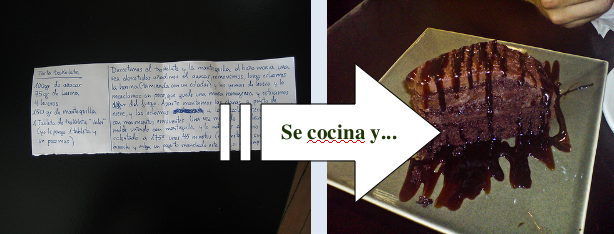
\includegraphics[width=0.8\textwidth]{./Utils/receta_pastel.png}              
                                                                \end{center}
       \end{frame}

\begin{frame}
 \frametitle{Algunas aplicaciones software libre}
 \begin{itemize}
  \item Sistema operativo Linux, diferentes distribuciones: K/Ubuntu, Fedora,
Red Hat, Debian, Suse, Mandriva...
    \item Navegadores web: Firefox, Chrome, etc.
    \item Procesador de textos: OpenOffice.
    \item Reproductores multimedia: VLC, Amarok...
    \item Hay programas libres para hacer pr\'acticamente de todo.
 \end{itemize}
 \begin{center}

\includegraphics[width=0.55\textwidth]{./Utils/Aplicaciones-libres.jpg}  
\end{center} 
\end{frame}

\subsection{?`Por qu\'e usarlo?}

\begin{frame}
 \frametitle{?`Por qu\'e usar software libre?}
 \begin{itemize}
  \item Porque garantiza nuestra libertad de elecci\'on, ahora y en el futuro.
  \begin{itemize}
    \item Dependencia tecnol\'ogica.
    \item Est\'andares.
    \end{itemize}
    \item Porque potencia la participaci\'on en proyectos de software.
    \item Porque favorece el desarrollo de empresas locales frente a las
multinacionales extranjeras.
 \end{itemize}
 \begin{center}

\includegraphics[width=0.55\textwidth]{./Utils/logo-esle.jpg}   \end{center}  
\end{frame}



\begin{frame}
 \frametitle{?`Por qu\'e usar software libre?}
 \begin{itemize}
\item Porque nos permite modificar la aplicaci\'on libremente y adecuarla a
nuestras necesidades.
\item Porque fomenta el uso de formatos abiertos y compatibilidad entre
aplicaciones.
\item Porque es un recurso de conocimiento para toda la humanidad que va
creciendo con el tiempo.
 \end{itemize}

\end{frame}

\subsection{?`D\'onde encontrarlo?}
\begin{frame}
 \frametitle{?`De d\'onde obtenemos software libre?}
 \begin{itemize}
\item Fundamentalmente de la web.
\item Tambi\'en de copias que nos proporcione alguien: es legal.
\item Si trabajas con GNU/Linux: repositorios.
\item P\'aginas de alternativas libres:
\begin{itemize}
\item \url{http://www.freealts.com/}
\item \url{http://www.osalt.com/}
\item
\begin{scriptsize}\url{
http://www.uca.es/softwarelibre/programas/alternativas_libres_docencia}        
\end{scriptsize}
 \end{itemize}
 \item Software libre para Windows: \url{http://www.cdlibre.org/}
\end{itemize}
\end{frame}

\subsection{C\'omo aprender}
\begin{frame}
 \frametitle{?`C\'omo aprendo a usar software libre?}
 \begin{itemize}
\item Hay muchos recursos en la web: cursos, manuales, blogs, foros...
\item Gran comunidad de usuarios que aporta documentaci\'on y soluciones.
\item Itsas: se puede pedir ayuda a trav\'es de la lista de correo.
\end{itemize}
\end{frame}

\section{Itsas}
\subsection{Participar}
\begin{frame}
 \frametitle{?`C\'omo puedo participar?}
 \begin{itemize}
\item Suscr\'ibete a nuestra lista de correo. Ah\'i podr\'as preguntar dudas y
aportar soluciones: \url{http://itsas.ehu.es/participate}
\item En la lista te enterar\'as de eventos que organicemos, novedades sobre
software libre, etc.
\item Enviar \texttt{subscribe} a \texttt{itsas-request@ehu.es}
\end{itemize}
\end{frame}

\subsection{Actividades}
\begin{frame}
 \frametitle{?`Qu\'e cosas se hacen en Itsas?}
 \begin{itemize}
\item Fomentar el uso del software libre en la universidad, e intentar que se
cumplan los formatos est\'andares. 
\item Organizar eventos relacionados con el software libre, como Install
Partys, cursos, charlas, etc. 
\item Evento reciente: Akademy-es 2010
(\url{http://www.kde-espana.es/akademy-es2010})
\end{itemize}
 \begin{center}

\includegraphics[width=0.35\textwidth]{./Utils/akademyes2010.png}  
\end{center} 

\end{frame}

\begin{frame}
 \frametitle{?`Qu\'e cosas se hacen en Itsas?}
 \begin{itemize}
\item Pr\'oximamente se organizar\'a una Install-Party, donde se ense\~nar\'a a
instalar K/Ubuntu, se resolver\'an dudas con software libre ya instalado, etc.
\item No es necesario tener conocimientos previos para asistir.
\item Si s\'i ten\'eis conocimientos, pod\'eis acercaros a ayudar, y compartir
conocimiento.
\item !`Suscrib\'ios a la lista y estad atentos!
\end{itemize}
\end{frame}

\begin{frame}[t]
\titlepage
\end{frame}

\end{document}
